\documentclass{beamer}

%style
\mode<presentation>
\usetheme{Boadilla}

%Einstellungen der Präsentation
\title[Offensive Security]{Fuzzing Methods}
\subtitle{Offensive Security}
\author{Moritz Rupp}
\institute[MR]{Hochschule Albstadt-Sigmaringen}
\setbeamertemplate{navigation symbols}{}%remove navigation symbols
\date{SS 22}

%Beginn der Präsentation
\begin{document}
\begin{frame}
 \titlepage
\end{frame}
\begin{frame}{Contents}
 \tableofcontents
\end{frame}
\section{Fuzzing background}
\begin{frame}{Fuzzing background}
\begin{itemize}
 \item Development produces bugs, errors and unintentionally behaviour
 \item Gateway for vulnabilities and exploits
 \item Software testing tries to oppose that
 \item Many different approaches exist
\end{itemize}
\end{frame}
\subsection{Software testing}
\begin{frame}{Software testing}
 \begin{block}{Manuel testing}
  - Code reviews, manuel search for vulnabilities\\
  - Time consuming, expensive
 \end{block}
\begin{block}{Static analysis}
- Automatically examine source code bevore the programm is run\\
- Pattern analysis \\
- Control flow graph, data flow analysis\\
- Expensive tooling
\end{block}
\begin{block}{Dynamic analysis}
- Automatically examine a programm while its's been run\\
- Execute and input data in real-time\\
\end{block}
\end{frame}
\subsection{Fuzz-testing}
\begin{frame}{Fuzz-testing}

  $\Rightarrow$ Fuzz-testing is the cutting edge of dynamic analysis
  
  \begin{itemize}
   \item Input data in real-time
   \item Monitor the system behaviour
   \item Listen for exceptions
   \item Provide feedback
  \end{itemize}

\end{frame}
\section{Functionality}
\begin{frame}{Functionality}
\begin{enumerate}
 \item Identify target interfaces\\
 - portscanning, code reviews
 \item Generate inputs\\
 - mutation, generation based fuzzing
 \item Feed these inputs to the target system
 \item Monitor for exceptions
 \item Log exceptions
\end{enumerate}

\end{frame}
\begin{frame}{Basic Fuzzing application}
\begin{center}
  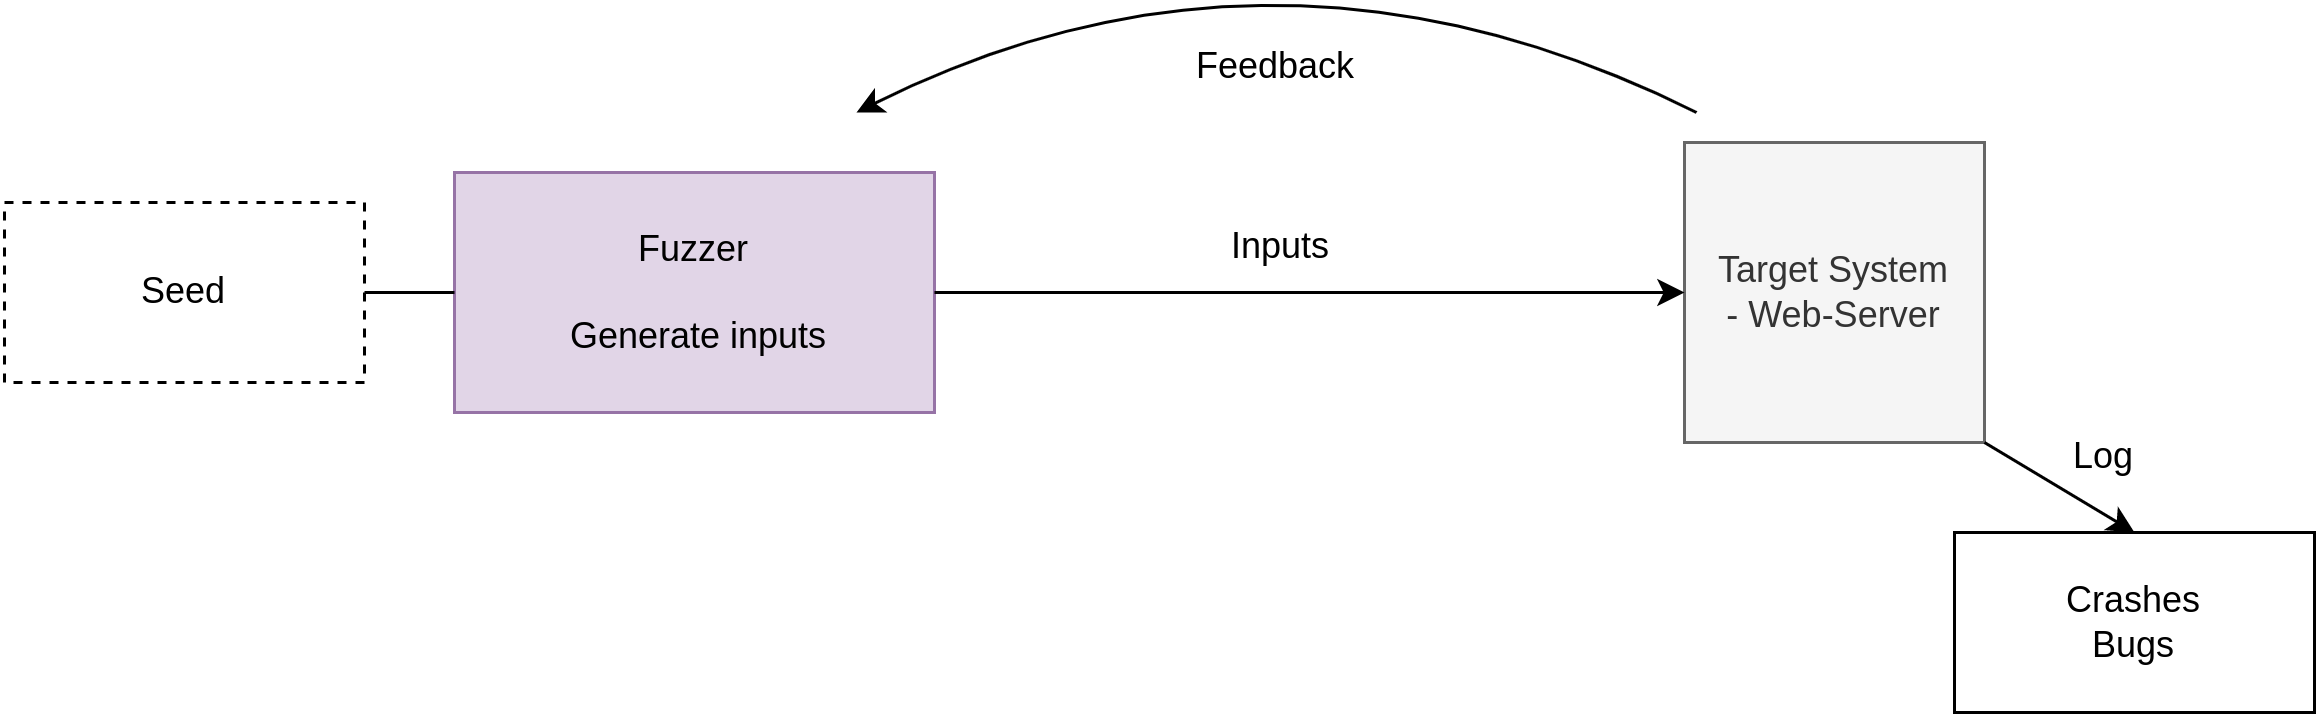
\includegraphics[scale=0.15]{basicfuzz.png}
\end{center}
\end{frame}
\begin{frame}{Fuzzing Methods}
 \begin{itemize}
  \item Huge landscape of applications and infrastructers\\
  - Web-applications, networks, binarys etc.\\
  $\Rightarrow$ No generall solution
  \item Different targets expect different inputs
  \item How do we generate those inputs?\\
  $\Rightarrow$ Mutation based fuzzing\\
  $\Rightarrow$ Generation based fuzzing
 \end{itemize}

\end{frame}
\begin{frame}{Mutation based Fuzzing}
\begin{itemize}
 \item Mutate already existing data
 \item Randomly or after fixed patterns
\end{itemize}

 
\end{frame}







\end{document}
